\section{Σύγκριση αποτελεσμάτων FD, DA, CA} 

\subsection{Σύγκριση τιμών παραγώγων}

\begin{table}[h!]
    \begin{center}
        \begin{tabular}[c]{|c|c|c|c|}
            \hline
            & FD & DA & CA \\
            \hline
            $\dfrac{\delta F}{\delta b_1}$ & -9.3e-6 & -6.9e-6 & -1.4e-5\\[8pt]
            $\dfrac{\delta F}{\delta b_2}$ & -1.1e-5 & -8.1e-6 & -7.8e-5\\[8pt]
            $\dfrac{\delta F}{\delta b_3}$ & -1.3e-5 & -9.9e-6 & 2.1e-6\\[8pt]
            \hline
        \end{tabular}
    \caption{Σύγκριση παραγώγων απο τις τρείς μεθόδους}
    \label{tab:finalComp}
    \end{center}
\end{table}

Αρχικά παρατηρείται πως αν και με κάθε μέθοδο οι παράγωγοι που προκύπτουν είναι στην ίδια τάξη μεγέθους, υπάρχουν αισθητές διαφορές στις τιμές τους, μάλιστα, για την τρίτη παράγωγο, η συνεχής συζηγής μέθοδος οδηγεί σε λύση με αντίθετο πρόσημο σε σχέση με τις άλλες δυο μεθόδους. 

Συγκεκριμένα, μπορούμε να αποφανθούμε πως οι τιμές των πεπερασμένων διαφορών και της διακριτής συζυγής μεθόδου είναι αρκετά κοντά, ωστόσο η συνεχής συζυγής μέθοδος απέχει περισσότερο απο τις άλλες δυο. Όπως αναφέραμε και στην προηγούμενη παράγραφο, αυτό πιθανότατα οφείλεται στην δεύτερη αριθμητική επίλυση της FAE με δεδομένα που προκύπτουν απο την αριθμητική επίλυση της primal εξίσωσης. Έτσι, είναι πολύ επηρεπής στη συσσώρευση σφαλμάτων, οπότε ίσως ήταν σκόπιμο να επιχειρούσαμε την αναλυτική επίλυσή της ή την επίλυσή της με κάποια άλλη μέθοδο για τον περιορισμό των σφαλμάτων. 

Αναφορικά με τις διαφορές στις τιμές των αποτελεσμάτων για τις πεπερασμένες διαφορές και τη διακριτή συζυγή μέθοδο, οι δύο μέθοδοι θα έπρεπε να οδηγούν σε πολύ κοντινότερα αποτελέσματα. Πιθανότατα, η διαφορά προκύπτει απο την έκφραση της παραγώγου ως πεπερασμένες διαφορές στην εξίσωση \ref{eq:pRUfinal}. Έγινε δοκιμή για αναπαράσταση ως κεντρικές διαφορές ωστόσο τα αποτελέσματα ήταν ελαφρώς χειρότερα. Στη διακριτή μέθοδο, οι άλλες δυο απαιτούμενες ποσότητες ($\dfrac{\partial \vec{R}}{\partial \vec{b}}$) και ($\dfrac{\partial F}{\partial \vec{U}}$) ελέγθηκαν συγκρίνωντας τις με τις αντίστοιχες παραγώγους που προκύπτουν απο πεπερασμένες διαφορές και οδηγούσαν σε ταυτόσημα αποτελέσματα. 

\subsection{Σύγκριση υπολογιστικού κόστους} 

Εκτός απο τις τιμές των παραγώγων στον παρακάτω πινακα (\ref{tab:cost}) παρατίθενται τα υπολογιστικά κόστη κάθε μεθόδου συγκριτικά με το κόστος επίλυσης του primal προβλήματος (1 primal = 1 TU).

   \begin{table}[h!]
    \begin{center}
        \begin{tabular}[c]{|r|l|}
            \hline
           FD & 6TU\\ 
           DA & 2TU\\ 
           CA & 2TU\\ 
            \hline
        \end{tabular}
    \caption{Σύγκριση υπολογιστικού κόστους των τριών μεθόδων}
    \label{tab:cost}
    \end{center}
   \end{table}
    
    
Φαίνεται λοιπόν, πως ο υπολογισμός με πεπερασμένες διαφορές (συγκεκριμένα με κεντρικές διαφορές) απαιτεί τριπλάσιο υπολογιστικό χρόνο συγκριτικά με τις άλλες δυο μεθόδους. Ωστόσο, εκφράζοντας τους υπολογιστικούς χρόνους απλά ως μονάδες χρόνου επίλυσης του primal προβλήματος δεν είναι τόσο ακριβής. Συγκεκριμένα, η DA απαιτεί την επίλυση γραμμικού συστήματος, που στην περίπτωσή μας (επίλυση με LU) ο χρόνος επίλυσης είναι ανάλογος του ($N^3$), ενώ μπορεί με άλλες μεθόδους συγκεκριμένα για τριδιαγώνια μορφή μητρώου συντελεστών να γίνει μέχρι και ανάλογος του ($N$). Επομένως, αφού λύνουμε το primal πρόβλημα με ρητό σχήμα, παρατηρήσαμε πως η DA ήταν αισθητά πιο αργή συγκριτικά με τις άλλες δυο μεθόδους, που δεν απαιτούν την επίλυση γραμμικού συστήματος. 

Στο παρακάτω σχήμα φαίνεται η εξάρτηση και των παραγώγων πλεον, απο το πλήθος των κόμβων. 

\begin{figure}[h!]
    \begin{center}
        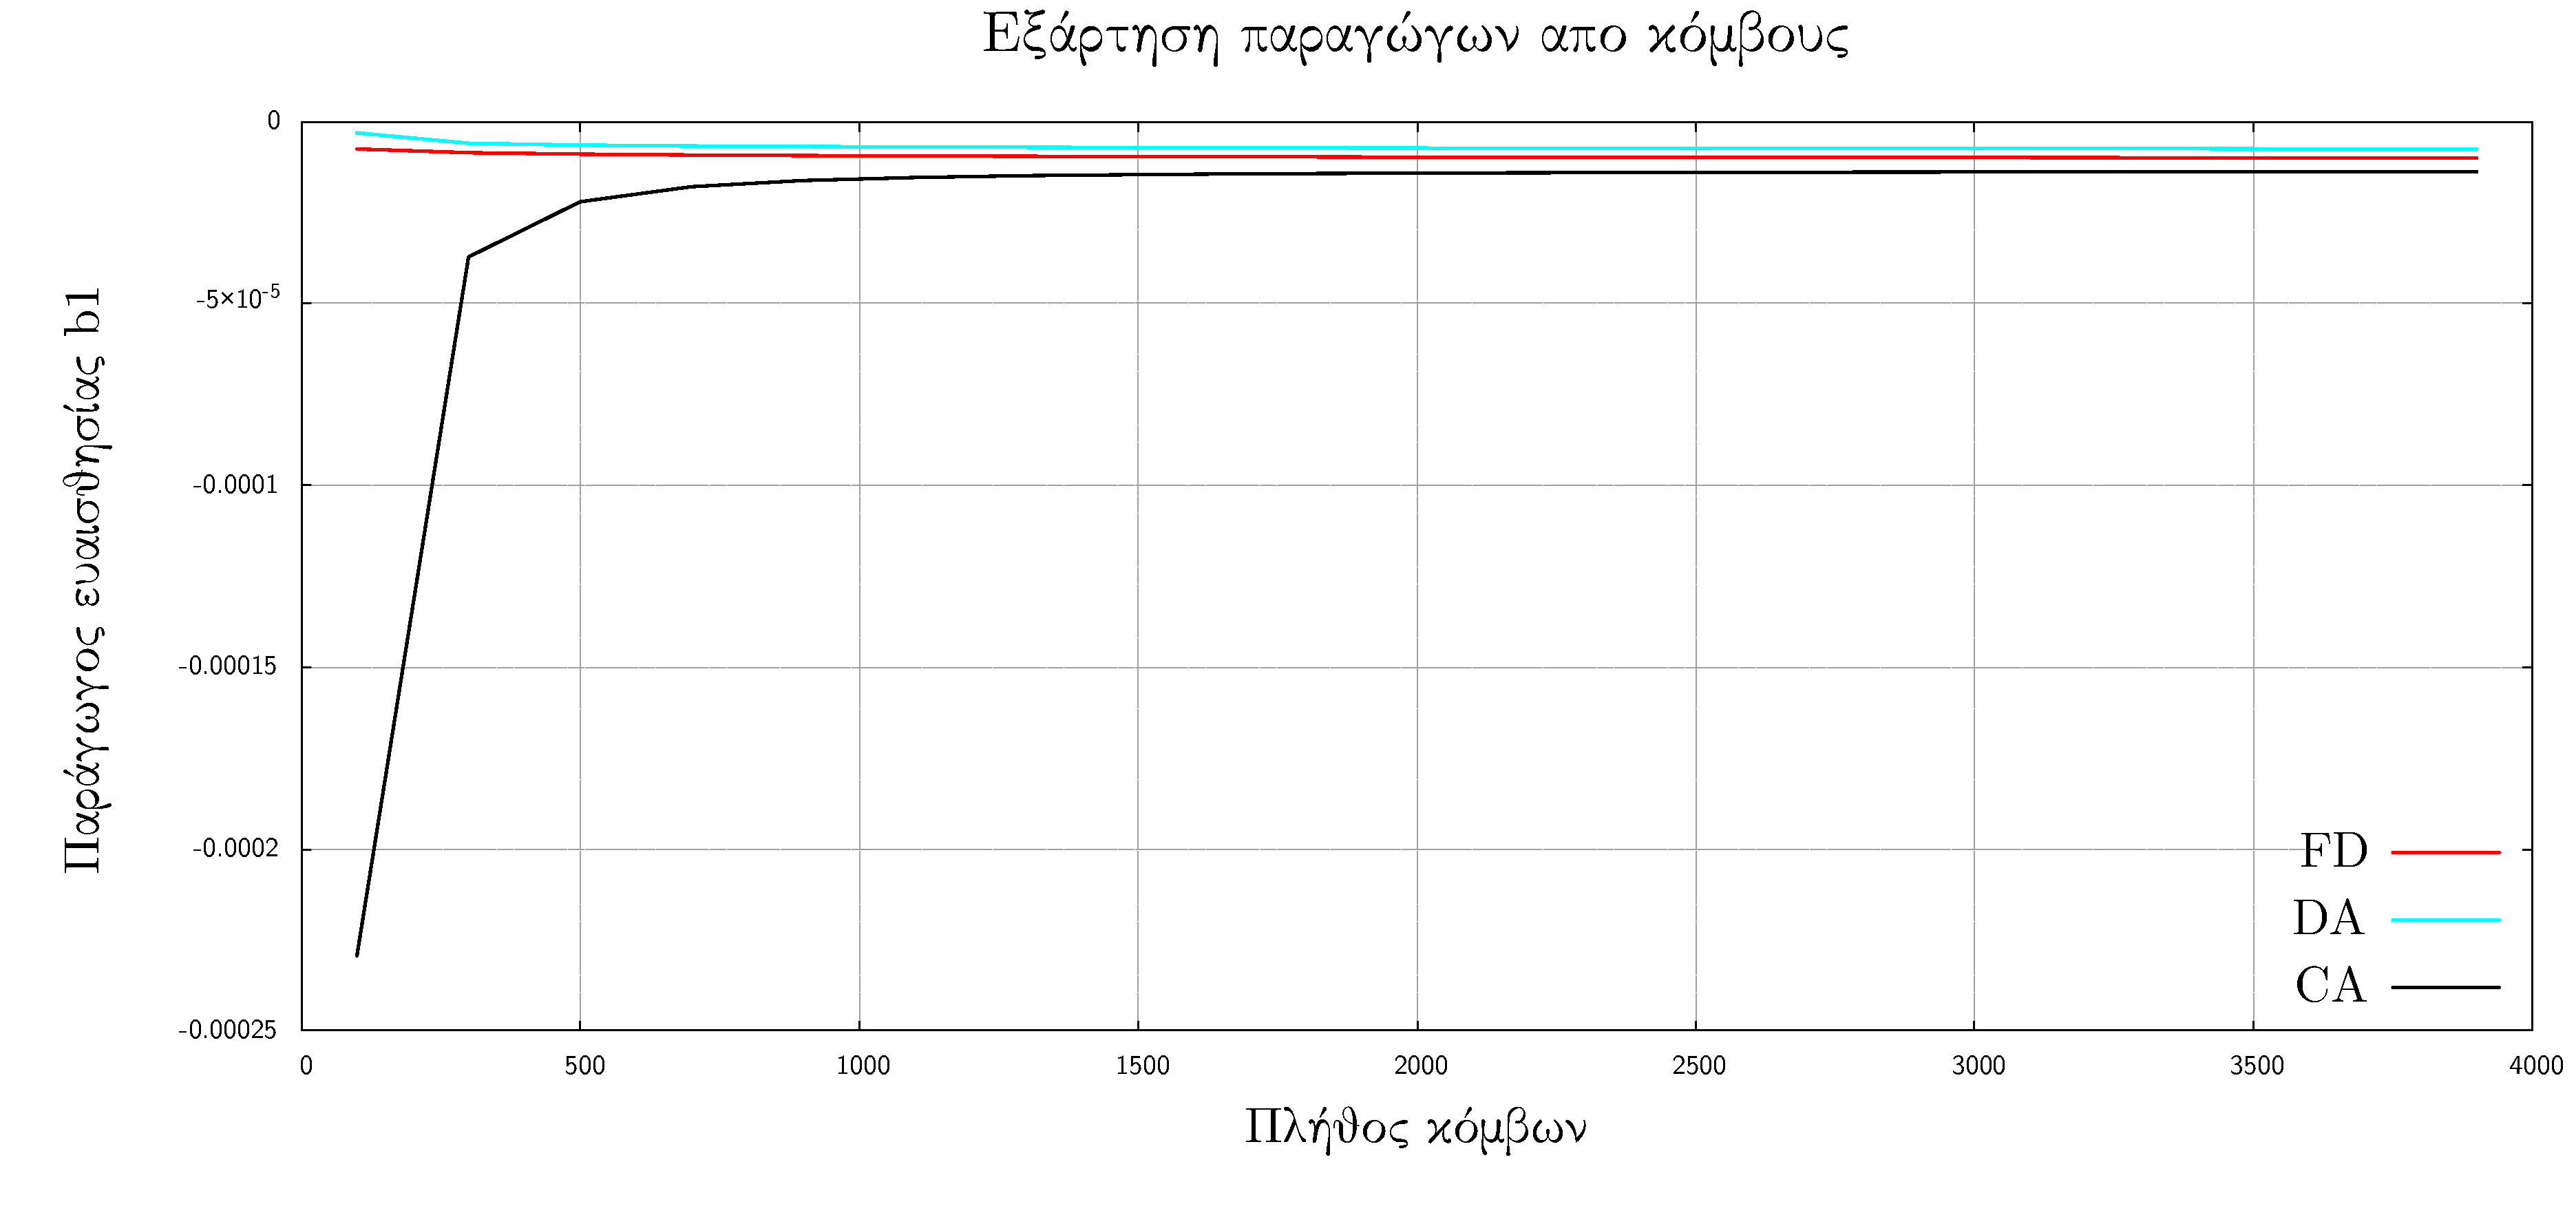
\includegraphics[width=0.95\textwidth]{figures/ders_vs_nodes.pdf}
    \end{center}
    \caption{Εξάρτηση παραγώγων απο τον αριθμό των κόμβων}
    \label{fig:der_vs_nodes}
\end{figure}

